% !TEX root = ../thesis.tex
\section{Porovnání člověk vs. stroj}
\label{chap:experiments:normalization}

Z experimentů provedených v části \ref{chap:experiments:analysis} vyplynula potřeba rozšířit korpus řečových dat. V části \ref{chap:experiments:analysis:reduction} se ukázalo, že v určitých případech jsou neznělé fonémy produkovány jako znělé. Pro lepší porozumnění tohoto jevu je nezbytné, aby řecový korpus obsahoval co možná nejvíce promluv obsahující slova slova s odlišným významem, ale lišící se pouze ve znělosti jedonho fonému.

Tato část se zaměřuje na získání takových to slov a experimentů s těmito slovy. Hlavním experimentem je porovnání schopností člověka tato slova od sebe odlišit a stroje. Na základě poznatků z tohoto experimentu jsou nabrženy úpravy, které mají sloužit k zlepšení systémů rozpoznávání řeči.

\subsection{Rozšíření řečového korpusu}
\label{chap:experiments:normalization:corpus}

Před samotným nahráváním bylo nezbytné vybrat co možná nejvíce dvojic slov, které se liší významem a ve znělosti právě jednoho fonému. Příkladem může být dvojice slov \textit{kosa} + \textit{koza} nebo \textit{přibít} + \textit{přibít}. Algoritmus výběru slov je následující:

\begin{enumerate}
  \item načtení dat (slovník, párové fonémy)
  \item shluknutí všech slov vedoucích ke stejné transckripci
  \item zkombinování všech transkripcí do dvojic
  \item nalezení dvojic transkripcí, které se liší právě ve znělosti jednoho fonému\footnote{Konkrétně algoritmus vzájemně porovná obě slova a najde rozdílné fonémy. Pokud tyto rozdíly odpovídají některé z dvojic párových fonémů, tak je dvojice přijata.}
  \item výběr dvojic slov na základě vybraných transkripcí
\end{enumerate}

Vstupem je tedy slovník obsahující slova a jejich fonetický přepis, dále pak dvojice fonémů (znělý + neznělý). Jako slovník posloužil seznam slov s fonetickými přepisy pocházející z jazykového modelu obsahující 1,2 milionu slov. Pomocí výše zmíněného algoritmu se podařilo nalézt $160$ párů slov lišících se znělostí právě jednoho fonému, celkem tedy $320$ slov. Ke každému nalezenému slovu byla následně vybrána minimálně jedna věta obsahující toto slovo (ale nikoli druhé slovo z dvojice), těchto vět je pak $418$. Příklad vybraných vět je níže

\begin{verbatim}
  Zkoušel jsem to několikrát, ale pokaždé padla kosa na kámen.
  Do basy nemusí, vlk žere, koza žije.
\end{verbatim}

Vybraná slova a věty jsou základem pro druhou etapu nahrávání. Nahrávání se zhostil stejný řečník jako v případě té první (viz část \ref{chap:experiments:analysis:corpus}). Samotné nahrávání bylo rozděleno do dvou samostatných sezení, mající mezi sebou týdenní rozestup. Oproti první etapě probíhalo nahrávání v odhlučněné nahrávácí komoře za pomocí profesionálního nahrávacího zařízení. Mikrofon byl od úst řečníka vzdálen přibližně 15 cm, protože byl použit studiový mikrofon, který kvůli své velikosti už z podstaty není možné přiložit přímo na tvář jako v případě první série nahrávání.

\begin{figure}[hbpt]
  \centering
  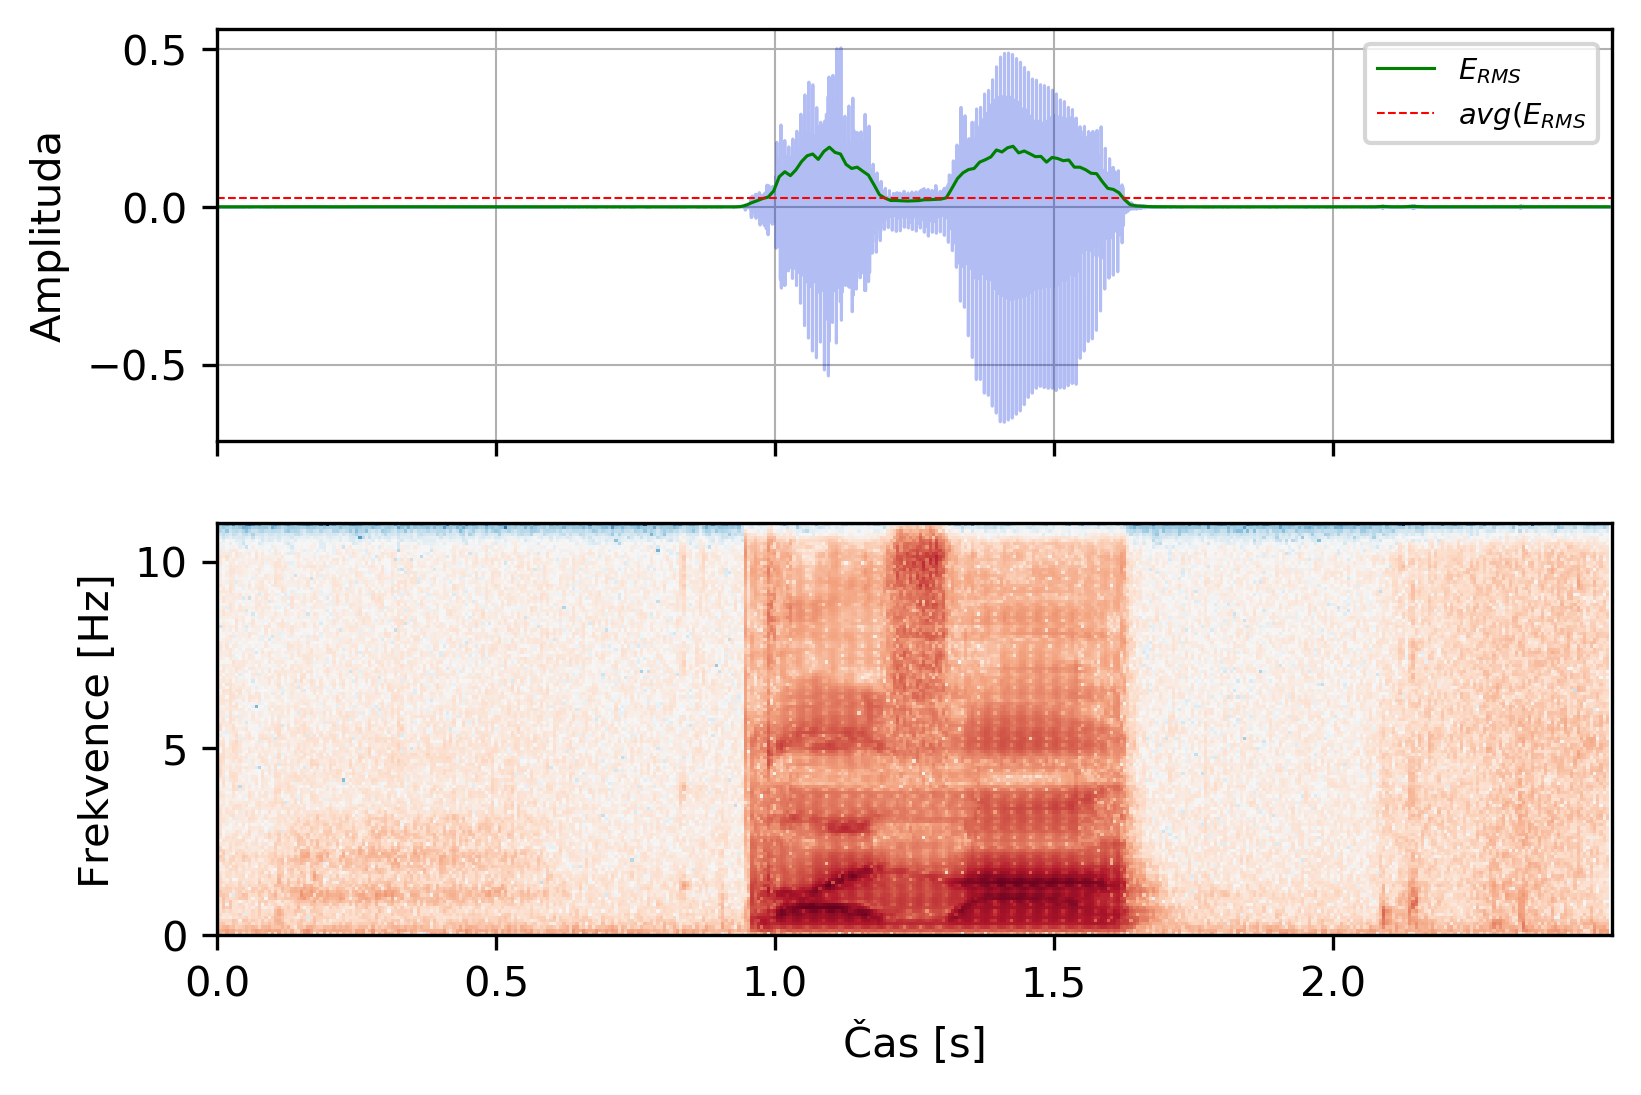
\includegraphics[width=0.9\textwidth]{./ch4-experiments/img/energy_spec_word.png}
  \caption{Průběh a spektrogram slova \uv{kosa} s společně s vyznačenou energií EL promluvy.}
  \label{fig:experiments:normalization:word}
\end{figure}

\begin{figure}[hbpt]
  \centering
  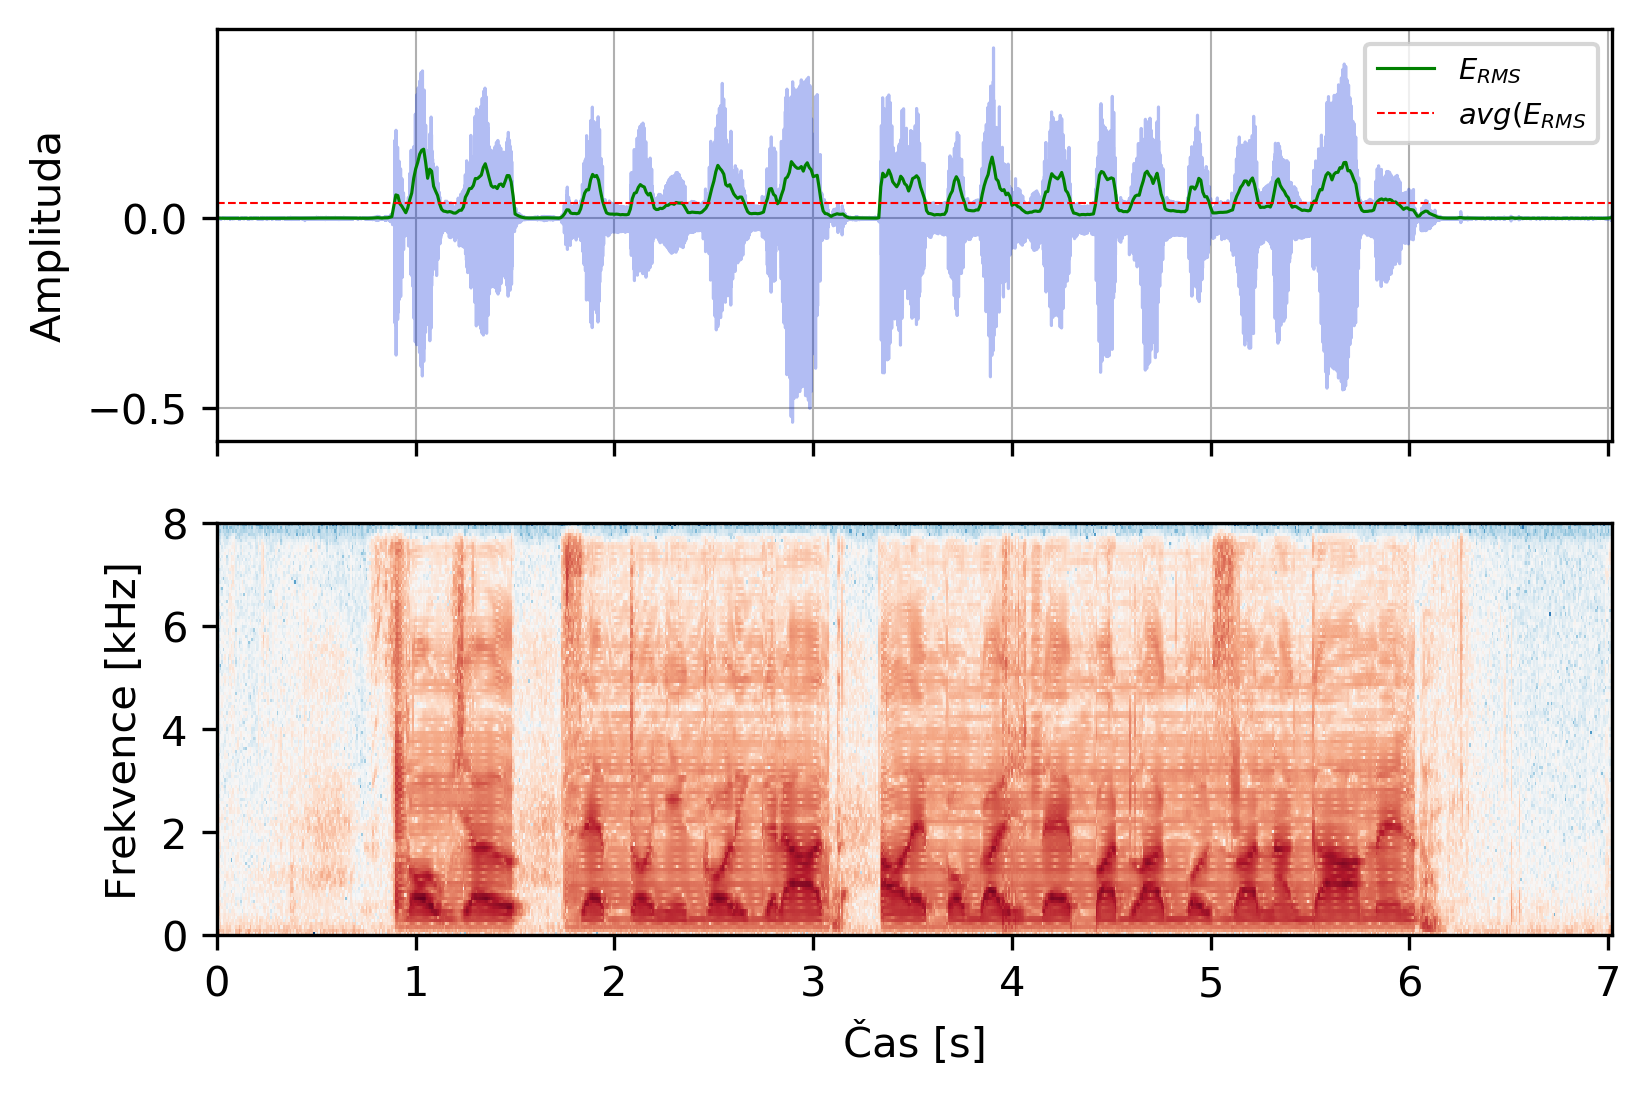
\includegraphics[width=0.9\textwidth]{./ch4-experiments/img/energy_spec_sentence.png}
  \caption{Průběh a spektrogram promluvy obsahující slovo \uv{kosa} a vyznačenou energií EL promluvy.}
  \label{fig:experiments:normalization:sentence}
\end{figure}

\subsection{Poslechový test}

\subsection{Výsledky porovnání}

\begin{itemize}
  \item popsat důvody proč potřebujeme další nahrávky (slova, která se liší znělostí)
  \item popsat algoritmus výberu slov/vět k nahrávání
  \item napsat něco o tom, že mezi nahráváními byl velký časový rozestup a taky se změnila technika nahráváními
  \item problém taky s tím, že první sada nahrávek je mnohem větší (10h) než ta nová (cca 30 min) a modely tak nefungovali na nových datech v testovací sade
  \item použití neuronovek (Kaldi)
  \item popis a výsledky experimentu \uv{člověk vs. stroj}
\end{itemize}
